\documentclass{article}

% if you need to pass options to natbib, use, e.g.:
%     \PassOptionsToPackage{numbers, compress}{natbib}
% before loading neurips_2019

% ready for submission
% \usepackage{neurips_2019}

% to compile a preprint version, e.g., for submission to arXiv, add add the
% [preprint] option:
%     \usepackage[preprint]{neurips_2019}

% to compile a camera-ready version, add the [final] option, e.g.:
     \usepackage[final]{neurips_2019}

% to avoid loading the natbib package, add option nonatbib:
%     \usepackage[nonatbib]{neurips_2019}

\usepackage[utf8]{inputenc} % allow utf-8 input
\usepackage[T1]{fontenc}    % use 8-bit T1 fonts
\usepackage{hyperref}       % hyperlinks
\usepackage{url}            % simple URL typesetting
\usepackage{booktabs}       % professional-quality tables
\usepackage{amsfonts}       % blackboard math symbols
\usepackage{nicefrac}       % compact symbols for 1/2, etc.
\usepackage{microtype}      % microtypography

\usepackage{amsmath,amssymb,amsfonts,amsthm}
\usepackage{graphicx}
\usepackage{bbm}
\usepackage{latexsym}
\usepackage{natbib}
\usepackage{multirow}

\newcommand{\Yten}{\pmb{Y}}
\newcommand{\subs}{\pmb{i}}
\newcommand{\wsu}[2]{#1_{\subs #2}}
\newcommand{\wsup}[2]{#1_{\subs}^{(#2)}}

% Aliases for some of the complicated y-indexing
\newcommand{\ytP}{\wsup{\tilde{y}}{+}}
\newcommand{\ytPM}{\wsup{\tilde{y}}{\pm}}
\newcommand{\ysk}{y_{\subs k}}
\newcommand{\ys}{y_{\subs}}
\newcommand{\ysh}{\hat{y}_{\subs}}
\newcommand{\taus}{\tau_{\subs}}
\newcommand{\lamP}{\wsup{\lambda}{+}}
\newcommand{\lamM}{\wsup{\lambda}{-}}
\newcommand{\lamPM}{\wsup{\lambda}{\pm}}
\newcommand{\gP}{\wsup{g}{+}}
\newcommand{\gM}{\wsup{g}{-}}
\newcommand{\gPM}{\wsup{g}{\pm}}
\newcommand{\factori}[1]{\theta^{(#1)}}
\newcommand{\mus}{\mu_{\subs}}
\newcommand{\musk}{\mu_{\subs k}}

\newcommand{\ms}{m_{\subs}}
\newcommand{\yvs}{\vec{\boldsymbol{y}}_{\subs}}
\newcommand{\yvtP}{\boldsymbol{\tilde{y}}_{\subs}^{(+)}}


% Commands for sampling
\newcommand{\Bess}[1]{\textup{Bessel}\left( #1 \right)}
\newcommand{\Binom}[1]{\textup{Binom}\left( #1 \right)}
\newcommand{\Exp}[1]{\textup{Exp}\left( #1 \right)}
\newcommand{\Gam}[1]{\textup{Gamma}\left( #1 \right)}
\newcommand{\Multi}[1]{\textup{Multinom}\left( #1 \right)}
\newcommand{\Skel}[1]{\textup{Skellam}\left( #1 \right)}
\newcommand{\Pois}[1]{\textup{Poisson}\left( #1 \right)}
\newcommand{\Geo}[1]{\textup{2SGeom}\left( #1 \right)}
\newcommand{\Delt}[1]{\mathbbm{1}\left( #1 \right)}

% Naming Bessel arguments
\newcommand{\besv}{order}
\newcommand{\besa}{coordinate}

% Expectations
\newcommand{\Eq}[1]{\mathbbm{E}_Q\left[#1\right]}
\newcommand{\Vq}[1]{\mathbbm{V}_Q\left[#1\right]}
\newcommand{\Gq}[1]{\mathbbm{G}_Q\left[#1\right]}
\newcommand{\E}[1]{\mathbbm{E}\left[#1\right]}
\newcommand{\V}[1]{\mathbbm{V}\left[#1\right]}
\newcommand{\G}[1]{\mathbbm{G}\left[#1\right]}

\newcommand{\Gqnot}[2]{\mathbbm{G}_{Q_{\backslash #1}}\left[#2\right]}
\newcommand{\Eqnot}[2]{\mathbbm{G}_{Q_{\backslash #1}}\left[#2\right]}

\newcommand{\given}{\,|\,}
\newcommand{\teq}{\!=\!}
\newcommand{\tp}{\!+\!}
\newcommand{\tm}{\!-\!}
\newcommand{\compcond}[1]{\big(#1\given-\big)}

% Spelling naive with the diacritical
\newcommand{\naive}{na\"{i}ve}
\newcommand{\Naive}{Na\"{i}ve}

\newtheorem{proposition}{Proposition}

% Set the typeface to Times Roman
\usepackage{times}

\title{Supplementary Information for A Variational Approach for Locally Private Inference of Poisson Factorization Models}

\author{} % LEAVE BLANK FOR ORIGINAL SUBMISSION.

% \author{\Name{Alexandra Schofield} \Email{xanda@cs.cornell.edu} \AND
% \Name{Aaron Schein} \Email{aschein@cs.umass.edu} \AND \Name{Zhiwei Steven Wu}
% \Email{zsw@umn.edu} \AND \Name{Hanna Wallach} \Email{hanna@dirichlet.net} }

\begin{document}

\maketitle

\section{The Bessel distribution as exponential family}
  \label{sec:expfambessel}
  
  We show that that with the $\nu$ parameter fixed, the Bessel distribution can be defined as an exponential family function.
  
  \textbf{Theorem 1}
    \label{theorem:expfam}
    \textit{The Bessel distribution $k \!\sim\!\textrm{Bes}(\nu, a)$ for fixed
   $\nu$ is an exponential family with sufficient statistic $T_\nu(k) \teq 2k
   \tp \nu$, natural parameter $\eta_\nu(k) \teq \log\left(\frac{a}{2}\right)$,
   and base measure $h_\nu(k) \teq \frac{1}{k!\,(k+\nu)!}$.}

   \begin{proof}
   The Bessel distribution \cite{yuan2000bessel} is a distribution whose support is the natural numbers:
     \begin{equation}
     f(k; a, \nu) = \frac{\left(\frac{a}{2}\right)^{2k+\nu}}{k!\, \Gamma(k + \nu + 1) I_\nu(a)}.
     \label{eq:besseldist}
     \end{equation}
   
   The name Bessel refers to the inclusion of $I_\nu(a)$, a modified Bessel function of the
     first kind:
     \begin{equation}
     I_\nu(a) = \sum_{n=0}^\infty
     \frac{\left(\frac{a}{2}\right)^{2n+\nu}}{n!\, \Gamma(n +\nu + 1)}.
       \end{equation}
   
   To qualify as an exponential family distribution, the probability mass function in Equation \ref{eq:besseldist} must factor into the following exponentiated structure:
   \begin{equation}
       pmf(x; \vec{\theta}) = h(x) e^{\eta(\theta) \dot T(x) - A(\theta)},
   \end{equation}
   where $x$ is the sampled value and $\theta$ are the distribution parameters.
   It is important that the natural parameters $\eta$ depend only on the parameters $\theta$, not the data, $x$.
   Similarly, the sufficient statistics, $T(x)$, reflect only the data and not the parameters.
   The function is normalized by a base measure $h(x)$ and a log partition $A(\theta)$.
   
   To put the Bessel function with fixed $\nu$ into an exponential family form, we need to factorize into terms depending only on $a$ and terms depending only on $k$.
   As we are treating $\nu$ as an integer constant instead of a parameter, we will rewrite the PMF as $f_{\nu}$ and replace the Gamma function with a factorial:
   
   \begin{equation}
       f_{\nu}(k; a) = \frac{\left(\frac{a}{2}\right)^{2k+\nu}}{k! (k + \nu)! I_\nu(a)}.
   \end{equation}
   
   We then separate out the terms into those depending on $a$, $k$, or both:
   
   \begin{equation}
       f_{\nu}(k; a) = (k!(k + \nu)!)^{-1} \cdot (I_{\nu}(a))^{-1} \cdot \frac{a}{2}^{2k + \nu}.
   \end{equation}
   
   We can take $h(k) = (k!(k + \nu)!)^{-1}$ to be the base measure,
   and exponentiate the rest:
   
   \begin{equation}
       f_{\nu}(k; a) = h(k) e^{(2k + \nu)(\log(a/2)) - \log(I_{\nu}(a)))}.
   \end{equation}
   
   From here, the other three functions fall out, giving the full form:
   
   \begin{align}
     h(k) &= (k!(k + \nu)!)^{-1} \\
     T(k) &= 2k + \nu \\
     \eta(a) &= \log\left(\frac{a}{2}\right) \\
     A(a) &= \log I_\nu(a).
   \end{align}
   
   This shows that with fixed $\nu$, the PMF $f_{\nu}(k; a)$ of the Bessel distribution is exponential family.
\end{proof}
  
\section{The mode and mean of the Bessel distribution}
\label{sec:besselmode}

\textbf{Proposition 3}
  \label{theorem:besselmode}
  \textit{The mode of a Bessel distribution for parameters $a, \nu$ can be a constant-bounded approximation of the mean:}

\[
  \big| \mathbbm{E}_{\Bess{m; \nu, a})}[m]  - \textup{mode} \left(\Bess{m; a, \nu} \right) \big|  \leq 1.  
\]

The intuitive meaning of this is that the mode of the Bessel distribution is
guaranteed to be one of the two integers closest to the mean of the
distribution. Given one of these two integers will always be the best integer
approximation of this number, we can also say that there cannot exist an
integer approximation of the mean of the Bessel that is strictly between the
mode and the mean of the Bessel distribution.

\begin{proof}
  A Bessel distribution takes two arguments, which we refer to as its \besv,
  $\nu$ and \besa, $a$. The distribution is defined as:

  \begin{align}
      p(x = n~&|~x \sim \Bess{\nu, a})\notag \\
      &= \frac{1}{I_{\nu}(a)n!\Gamma(n + \nu + 1)} \left( \frac{a}{2} \right)^{2n + \nu},   
  \end{align}
  where $I_{\nu}(a)$ is a modified Bessel function of the first kind. The
  arithmetic mean of the distribution is
  \[
      \mathbbm{E}_{\Bess{m; \nu, a})}[m] = \frac{a}{2} R_{\nu}(a),
  \]
  with $R_{\nu}(a)$ referring to the ratio of two Bessel functions:
  \[
      \frac{I_{\nu + 1}(a)}{I_{\nu}(a)}.
  \]

  The Bessel distribution has one or two neighboring integer modes. The mode can
  be computed directly from the parameters of the distribution without Bessel
  functions:
  \[
      \textup{mode}(\Bess{\nu, a}) = \bigg \lfloor \frac{\sqrt{a^2 + \nu^2} - \nu}{2} \bigg \rfloor.
  \]
  Unlike the mean, which can take arbitrary non-negative real values, the mode
  is guaranteed by the floor function to be a non-negative integer.

  We use the following bound on the mean of a Bessel ratio from
  \citet{devroye2002simulating}

  \begin{equation}
      \frac{a}{\nu + 1 + \sqrt{a^2 + (\nu + 1)^2}} \leq R_{\nu}(a)
      \leq \frac{a}{\nu + \sqrt{a^2 + \nu^2}}.
  \end{equation}

  We multiply through by $\frac{a}{2}$ to bound the mean of the Bessel
  distribution:

  \begin{equation}
      \frac{a^2}{2(\nu + 1 + \sqrt{a^2 + (\nu + 1)^2})} \leq \mathbbm{E}_{\Bess{m; \nu, a})}[m]
      \leq \frac{a^2}{2(\nu + \sqrt{a^2 + \nu^2})}.
  \end{equation}

  We can rewrite these bounds using a difference-of-squares:

  \begin{align*}
      \frac{a^2}{2(\nu + \sqrt{a^2 + \nu^2})} &= 
      \frac{a^2(\sqrt{a^2 + \nu^2} - \nu)}{2(\nu + \sqrt{a^2 + \nu^2})(\sqrt{a^2 + \nu^2} - \nu)} \\
      &= \frac{a^2(\sqrt{a^2 + \nu^2} - \nu)}{2a^2 + \nu^2 - \nu^2} \\
      &= \frac{\sqrt{a^2 + \nu^2} - \nu}{2}.
  \end{align*}

  This upper bound coincides with the unrounded formulation of the mode. Because
  the mode is the floor of this quantity, we know it is less than or equal to
  this upper bound with a difference of less than 1.

  We can convert the lower bound in the same way:
  \begin{equation*}
      \frac{a^2}{2((\nu + 1) + \sqrt{a^2 + (\nu^2 + 1)})} =  \frac{\sqrt{a^2 + (\nu + 1)^2} - (\nu + 1)}{2}.
  \end{equation*}

  We are interested in bounding the difference between the upper and lower
  bounds:
  \begin{equation}
      \frac{\sqrt{a^2 + \nu^2} - \nu}{2} - \frac{\sqrt{a^2 + (\nu + 1)^2} - (\nu + 1)}{2} = 
      \frac{\sqrt{a^2 + \nu^2} + 1 - \sqrt{a^2 + (\nu + 1)^2}}{2}.
  \end{equation}

  Knowing that $\nu$ is positive, we can state that $\sqrt{a^2 + \nu^2} <
  \sqrt{a^2 + (\nu + 1)^2}$, or $\sqrt{a^2 + (\nu + 1)^2} - \sqrt{a^2 + \nu^2} >
  0$. Based on the upper slice of the triangle in the figure below, the triangle
  inequality also gives us another bound, that $\sqrt{a^2 + \nu^2} + 1 >
  \sqrt{a^2 + (\nu + 1)^2}$, or $1 > \sqrt{a^2 + (\nu + 1)^2} - \sqrt{a^2 +
  \nu^2}$.

  \begin{center}
  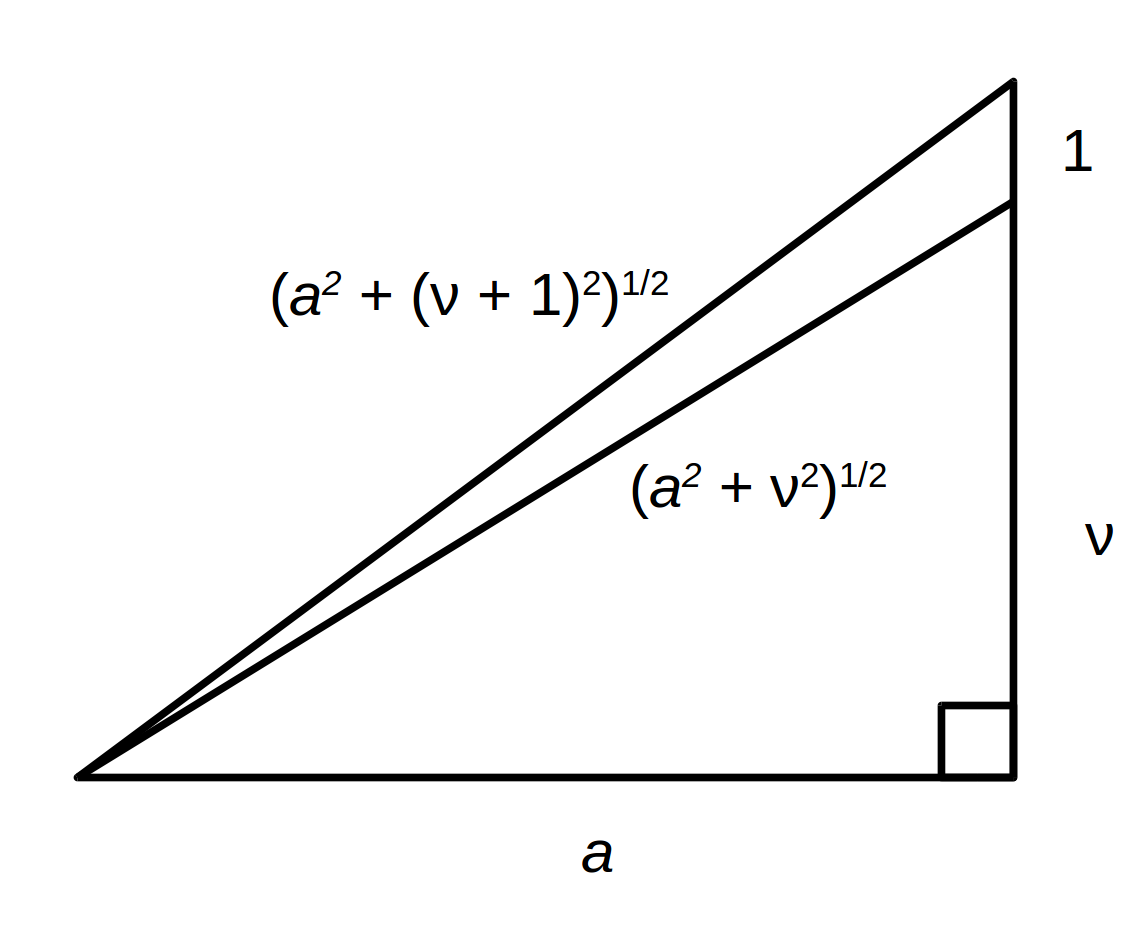
\includegraphics[width=0.3\textwidth]{figures/triangle-bessel-model}
  \end{center}
  Together, these imply that 
  \[
      0 \leq \sqrt{a^2 + \nu^2} + 1 - \sqrt{a^2 + (\nu + 1)^2} \leq 1.
  \]

  Substituting this in to our computation of the distance between the upper and
  lower bounds of the mean, we find that
  \begin{equation}
  \frac{\sqrt{a^2 + \nu^2} + 1 - \sqrt{a^2 + (\nu + 1)^2}}{2} < \frac{1}{2},
  \end{equation}

  or that the inferred upper and lower bounds for the mean of the Bessel
  distribution produce an interval no larger than $\frac{1}{2}$. The upper bound
  of this $\frac{1}{2}$ interval is the same as the upper bound of the length-1
  open interval of the mode of the Bessel. In the most extreme case when the
  mode is at the bottom end of its range and the mean is at the top, we have
  \[
      \mathbbm{E}_{\Bess{m; \nu, a})}[m] - \textup{mode}(\Bess{\nu, a}) < 1.
  \]
  In the opposite case, we have
  \[
      \textup{mode}(\Bess{\nu, a}) - \mathbbm{E}_{\Bess{m; \nu, a})}[m] \leq \frac{1}{2} < 1.
  \]
\end{proof}

\bibliographystyle{plainnat}
\bibliography{neurips_2019}
  
\end{document}
